\chapter{Background and Literature Review}\label{ch:background}

\section{Introduction}\label{sec:bg-intro}
This chapter reviews the field in which the thesis is placed. Section~\ref{sec:bg-mot} gives an overview of multi-object tracking: its evolution, its applications and challenges, its real-time constraints, a formal definition of tracking by detection, and its main paradigms. Section~\ref{sec:bg-detectors} reviews object detectors and the meaning and calibration of their confidence scores, and Section~\ref{sec:bg-trackers} reviews the tracking-by-detection trackers used in this work and how they use these scores. Section~\ref{sec:bg-datasets} introduces the datasets of the field. Section~\ref{sec:bg-review} reviews the work closest to the two proposed controllers, summarizes it in a comparison table, and states the gap that the thesis addresses. Sections~\ref{sec:bg-mot}--\ref{sec:bg-datasets} extend the survey published by the author in \cite{ismail2026realtime}.

\section{Multi-Object Tracking Overview}\label{sec:bg-mot}

\subsection{Evolution of Object Detection and Tracking}\label{sec:bg-evolution}
Object detection and tracking have evolved through three technological phases \cite{li2025motreview}. Before 2012, detectors relied on hand-engineered features such as the histogram of oriented gradients \cite{dalal2005hog} and scale-invariant keypoints \cite{lowe2004sift}, combined with sliding windows and shallow classifiers. The second phase began when convolutional neural networks (CNNs) trained on large labelled datasets \cite{krizhevsky2017alexnet,russakovsky2015imagenet} outperformed hand-crafted features; region-based detectors \cite{girshick2014rcnn,ren2017fasterrcnn} and single-stage detectors \cite{redmon2016yolo,liu2016ssd} pushed the accuracy--speed frontier, and deep residual networks \cite{he2016resnet} became standard backbones. The third phase, beginning around 2020, introduced attention-based models \cite{vaswani2017attention,dosovitskiy2021vit}. The detection transformer (DETR) \cite{carion2020detr} removed anchors and NMS, and transformer-based trackers \cite{sun2020transtrack,meinhardt2022trackformer,zeng2022motr} integrated detection and association in one network.

Throughout these phases, multi-object tracking has been dominated by tracking by detection, whose trackers consume the output of an independent detector \cite{bewley2016sort,zhang2022bytetrack}. This thesis works within that paradigm, because it is the one in which detectors and trackers are combined and exchanged independently, and therefore the one in which their operating points must be reconciled.

\subsection{Applications and Challenges}\label{sec:bg-challenges}
Real-time detection and tracking are required wherever a system must perceive its environment continuously. Surveillance and security systems detect abnormal behavior and track people and vehicles in live streams. Driver assistance and autonomous driving rely on real-time detection of pedestrians, vehicles, and obstacles \cite{geiger2012kitti}. UAVs apply detection and tracking in traffic monitoring, inspection, search, and defense \cite{zhu2022visdrone,bakirci2025lowpower}, and the aerospace literature has studied airborne target tracking \cite{miller2015multitarget,desai2017uavfeature}, onboard deep detection \cite{lu2024uavdetection,choi2022docking}, and vision-based guidance \cite{parsons2019refueling}.

In crowded scenes, individual objects are hard to separate, and occlusion causes missed detections and identity switches. Fast motion, deformation, and long disappearance require motion models and appearance cues that remain reliable over many frames. Small objects, common in aerial footage, produce few pixels and low detector confidence \cite{cheng2023smallobject}. Illumination changes, blur, and weather reduce the detector's recall and change the distribution of its confidence scores \cite{chae2024radar}. Multi-object tracking therefore faces three coupled problems: detecting the objects, associating detections across frames, and keeping identities through occlusion \cite{li2025motreview}.

\subsection{Real-Time Constraints}\label{sec:bg-realtime}
Real-time performance is limited by three factors \cite{bakirci2025lowpower}. The first is the accuracy--speed trade-off: more accurate models generally need more computation and longer inference. The second is the hardware, which ranges from data-center graphics processing units (GPUs) to low-power embedded processors on board a vehicle or an aircraft. The third is the deployment context: bandwidth, power supply, and the need for onboard rather than remote processing. For a tracking pipeline these constraints act mainly through the detector, whose input resolution sets most of the cost; the tracker itself is usually inexpensive. A controller that changes the detector's resolution therefore also changes the cost of the pipeline, and a controller placed between the detector and the tracker must itself be cheap.

\subsection{Formal Definition of Tracking by Detection}\label{sec:bg-problem}
Let a video be a sequence of frames $\{I_t\}_{t=1}^{T}$. A detector estimates, for each frame, a set of candidates
\begin{equation}
\mathcal{D}_t = \{(\mathbf{x}_{t,i}, s_{t,i}, c_{t,i})\}_{i=1}^{n_t},
\label{eq:bg-dets}
\end{equation}
where $\mathbf{x}_{t,i}$ is a bounding box, $s_{t,i}\in(0,1)$ a confidence score, and $c_{t,i}$ a class label. Multi-object tracking associates detections across time into trajectories $\mathcal{T}=\{\tau_j\}$, each a sequence of boxes between a start frame and an end frame. An online tracker solves, frame by frame, an assignment problem
\begin{equation}
\pi_t^{*} = \arg\min_{\pi_t} \sum_{(i,j)\in\pi_t} C\left(\mathbf{x}_{t,i}, \tau_j\right),
\label{eq:bg-assign}
\end{equation}
where $\pi_t$ is a one-to-one matching between the detections of frame $t$ and the existing tracks, and $C$ is a cost based on predicted motion, appearance, or learned embeddings. The Hungarian method \cite{kuhn1955hungarian} solves this assignment exactly, and a Kalman filter \cite{kalman1960} is the usual motion predictor.

Two families of thresholds enter this formulation, and they are the subject of this thesis. The detector keeps only candidates whose score exceeds its confidence threshold and suppresses candidates that overlap a higher-scoring candidate by more than its NMS threshold, after resizing the frame to its input resolution. The tracker then admits detections to association and to track birth only above its own score thresholds. The quality of $\mathcal{T}$ therefore depends not only on the detector and the tracker, but also on whether their thresholds fit the scenes and the score distribution that the detector actually produces.

\subsection{Multi-Object Tracking Paradigms}\label{sec:bg-paradigms}
\emph{Tracking by detection.} A detector is applied independently to every frame, and an online tracker associates the detections over time using motion and appearance cues \cite{bewley2016sort,wojke2017deepsort}. The paradigm benefits directly from advances in detectors and remains modular: any detector can feed any tracker. It is the paradigm used throughout this thesis.

\emph{Joint detection and tracking.} JDE learns detection and appearance embeddings in a shared model \cite{wang2020jde}; FairMOT treats detection and re-identification (ReID) as equally important tasks with an anchor-free design \cite{zhang2021fairmot}; CenterTrack predicts object centers and their displacements between frames \cite{zhou2020centertrack}. These methods reduce the cost of a separate appearance model, but they couple the detector and the tracker, so that neither can be exchanged independently.

\emph{Transformer-based tracking.} TransTrack propagates queries between frames \cite{sun2020transtrack}; TrackFormer separates object queries for new objects from track queries for existing ones \cite{meinhardt2022trackformer}; MOTR carries track queries across frames and updates them by attention \cite{zeng2022motr}; MOTIP predicts identities directly \cite{gao2025motip}. These methods are fully differentiable, but they remain computationally expensive, and their thresholds are internal to the network.

\section{Object Detectors}\label{sec:bg-detectors}
Object detectors are broadly divided into two-stage and single-stage architectures, with transformer-based detectors forming a third group. Table~\ref{tab:bg-detectors} summarizes the detectors discussed in this section.

\subsection{Two-Stage Detectors}
The region-based CNN family first proposes candidate regions and then classifies and refines them \cite{girshick2014rcnn}. Faster R-CNN introduced a region proposal network that shares convolutional features with the detection head, which made the proposals nearly free and improved both speed and accuracy \cite{ren2017fasterrcnn}. Mask R-CNN added a parallel branch that predicts a segmentation mask for each detection \cite{he2017maskrcnn}. Two-stage detectors are accurate, particularly for small objects and cluttered scenes, but they are generally slower than single-stage detectors.

\subsection{Single-Stage Detectors}
Single-stage detectors predict boxes and class probabilities in one pass over the image. The YOLO (You Only Look Once) family treats detection as a regression problem over a grid \cite{redmon2016yolo}; successive versions improved the backbone, the neck, and the training recipe \cite{redmon2018yolov3,bochkovskiy2020yolov4,ge2021yolox,wang2024yolov9}, and recent generations distributed as software libraries, such as YOLOv8 \cite{jocher2023yolov8} and YOLO11 \cite{jocher2024yolo11}, offer a range of model sizes. The Single Shot MultiBox Detector (SSD) predicts boxes from feature maps at several scales \cite{liu2016ssd}. RetinaNet introduced the focal loss to address the imbalance between foreground and background during the training of dense detectors \cite{lin2017focal}. EfficientDet combined a bidirectional feature pyramid with compound scaling of resolution, depth, and width \cite{tan2020efficientdet}. Feature pyramid networks \cite{lin2017fpn} are the standard architectural response to scale variation in all of these detectors.

\subsection{Transformer-Based Detectors}
DETR formulates detection as set prediction with a transformer encoder--decoder, which removes anchors and NMS \cite{carion2020detr}. The original DETR converges slowly and is expensive. Real-time transformer detectors such as RT-DETR \cite{zhao2024rtdetr} and RF-DETR \cite{robinson2025rfdetr} keep the set-prediction formulation while reducing latency to the range of single-stage detectors.

\begin{table}[tbp]
\centering
\caption{Detector families discussed in this thesis. The last column indicates the thresholds that the user chooses when the detector is run.}
\label{tab:bg-detectors}
\begin{tabular}{>{\raggedright\arraybackslash}p{3.3cm}>{\raggedright\arraybackslash}p{1.0cm}>{\raggedright\arraybackslash}p{2.3cm}>{\raggedright\arraybackslash}p{5.2cm}>{\raggedright\arraybackslash}p{2.6cm}}
\toprule
Detector & Year & Architecture & Key idea & User thresholds \\
\midrule
R-CNN \cite{girshick2014rcnn} & 2014 & two-stage & CNN features on region proposals & confidence, NMS \\
Faster R-CNN \cite{ren2017fasterrcnn} & 2017 & two-stage & shared region proposal network & confidence, NMS \\
Mask R-CNN \cite{he2017maskrcnn} & 2017 & two-stage & parallel mask branch & confidence, NMS \\
YOLO \cite{redmon2016yolo} & 2016 & single-stage & grid regression of boxes and classes & confidence, NMS \\
SSD \cite{liu2016ssd} & 2016 & single-stage & multi-scale default boxes & confidence, NMS \\
RetinaNet \cite{lin2017focal} & 2017 & single-stage & focal loss for class imbalance & confidence, NMS \\
EfficientDet \cite{tan2020efficientdet} & 2020 & single-stage & bidirectional pyramid, compound scaling & confidence, NMS \\
YOLOX \cite{ge2021yolox} & 2021 & single-stage & anchor-free, decoupled head & confidence, NMS \\
DETR \cite{carion2020detr} & 2020 & transformer & set prediction, no NMS & confidence \\
RT-DETR \cite{zhao2024rtdetr} & 2024 & transformer & real-time hybrid encoder & confidence \\
\bottomrule
\end{tabular}
\end{table}

\subsection{Detector Confidence and Calibration}\label{sec:bg-confidence}
A classifier is calibrated when its confidence equals its probability of being correct. Modern neural networks are often poorly calibrated \cite{guo2017calibration}, and object detectors are no exception: their confidence depends on the position and size of the box as well as on the class, and it shifts with the data \cite{kuppers2020detcalib}. Detectors of different families \cite{redmon2016yolo,ren2017fasterrcnn,carion2020detr,zhao2024rtdetr,wang2024yolov9} produce different score distributions, and soft suppression changes the score of overlapping boxes \cite{bodla2017softnms}. The same object may therefore receive 0.9 from one detector and a much lower score from another. Calibration methods fit a mapping from scores to probabilities on labelled data \cite{kuppers2020detcalib}. That is not possible when a detector is exchanged in a deployed pipeline without labels. Test-time adaptation methods adapt a model to unlabelled data \cite{wang2021tent}, but they change the model's weights, whereas this thesis keeps both the detector and the tracker frozen.

Classical image thresholding offers a different tool. Otsu's method \cite{goh2018otsu} chooses, without labels, the threshold that best splits a histogram into two groups. For a candidate threshold $k$, let $\omega_0(k)$ and $\omega_1(k)$ be the fractions of values below and above $k$, and $\mu_0(k)$ and $\mu_1(k)$ their means. The method selects
\begin{equation}
k^{*}=\arg\max_{k}\;\omega_0(k)\,\omega_1(k)\,\bigl(\mu_0(k)-\mu_1(k)\bigr)^2,
\label{eq:bg-otsu}
\end{equation}
the threshold that maximizes the between-class variance. It needs no labels and adapts to the shape of the distribution. The self-calibrating layer of Chapter~\ref{ch:proposed} applies it to the logits of recent detector scores.

\section{Tracking-by-Detection Trackers}\label{sec:bg-trackers}
This section reviews the trackers that are used or discussed in the thesis, with attention to how each one uses detector scores. Table~\ref{tab:bg-trackers} summarizes them.

\subsection{Motion-Based Trackers}
SORT combines a constant-velocity Kalman filter with Hungarian assignment on box overlap \cite{bewley2016sort}. It is simple and fast, but it relies on motion alone, so occlusion and irregular motion cause many identity switches. The IOU tracker shows how far pure overlap association can go at high frame rates \cite{bochinski2017iou}. ByteTrack introduced a second association step: detections above a high threshold are associated first, and the tracks that remain unmatched are then associated with low-confidence detections, which recovers partially occluded objects that other trackers discard \cite{zhang2022bytetrack}. OC-SORT refines the Kalman filter with an observation-centric re-update and a velocity-direction consistency term, which improves robustness to occlusion and non-linear motion \cite{cao2023ocsort}; it uses a single confidence threshold. Buffered IoU matching enlarges the boxes during association to handle irregular motion \cite{yang2023cbiou}.

\subsection{Motion and Appearance Trackers}
DeepSORT adds deep appearance embeddings to SORT and combines the Kalman prediction with the cosine distance between embeddings, which reduces identity switches \cite{wojke2017deepsort}. BoT-SORT adds camera-motion compensation, an improved Kalman state, and ReID features to the ByteTrack association \cite{aharon2022botsort}. StrongSORT revisits DeepSORT with an exponential moving average of appearance features, camera-motion compensation by the enhanced correlation coefficient \cite{evangelidis2008ecc}, and other refinements \cite{du2023strongsort}. Deep OC-SORT adds adaptive appearance re-identification to OC-SORT \cite{maggiolino2023deepocsort}, and SMILEtrack learns similarity for occlusion-aware association \cite{wang2024smiletrack}. Many recent trackers improve association further with trained or domain-specific parts \cite{li2024fdbtrack,bao2024graphmatching,zhang2025sinkhorn,ding2025remot,liang2024motiontrack,sun2026bsr}; these change or retrain the tracker.

\subsection{Recent Trackers Used in This Thesis}
Hybrid-SORT uses weak cues, such as the confidence state and the height of a box, alongside strong cues \cite{yang2024hybridsort}. SparseTrack decomposes crowded scenes by pseudo-depth before association \cite{liu2025sparsetrack}. BoostTrack boosts the confidence of likely true detections and augments the similarity measure \cite{stanojevic2024boosttrack}. PD-SORT adds pseudo-depth cues to the motion model to handle occlusion \cite{wang2025pdsort}. U2MOT is an uncertainty-aware tracker trained without identity labels \cite{liu2023u2mot}. OATrack \cite{qi2026oatrack} is a recent tracker for small objects in UAV video; it weights association by detection quality, uses a YOLO detection cache, and has a fixed tracker-side confidence gate.

\subsection{How Trackers Use Detector Scores}\label{sec:bg-score-use}
All of these trackers read detector scores through fixed thresholds that their authors tuned for one detector, usually YOLOX \cite{ge2021yolox} on MOT17. Two kinds of trackers can be distinguished (Fig.~\ref{fig:bg-stages}). A \emph{single-stage} tracker, such as OC-SORT, ignores every box below one threshold. A \emph{two-stage} tracker, such as ByteTrack, uses boxes above a high threshold to match tracks and boxes above a higher threshold to start tracks, and it uses lower-score boxes, down to a low threshold, in a second step that can only continue tracks left unmatched by the first step. If a detector gives scores on a different scale from the one the thresholds were tuned for, a single-stage tracker can lose most of its boxes, and a two-stage tracker can lose its ability to start tracks. The published comparison in \cite{ismail2026realtime} shows the steady progress of tracking accuracy from motion-only methods to trackers that combine motion, appearance, and low-score association; it does not, and no leaderboard does, show how a tracker behaves when its detector changes.

\begin{figure}[tbp]
\centering
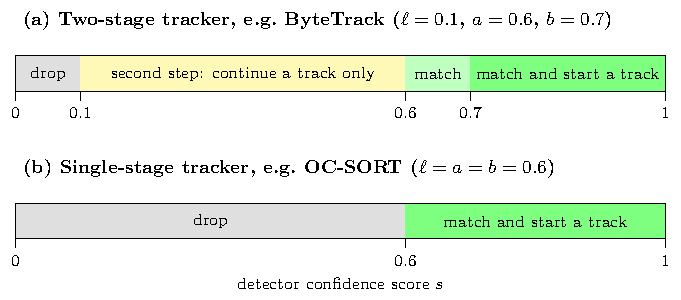
\includegraphics[width=0.9\textwidth]{figures/score_stages.pdf}
\caption{How a two-stage and a single-stage tracker use the detector score, with the published thresholds of ByteTrack (official setting) and OC-SORT. $\ell$: lowest score used; $a$: score needed to match a track; $b$: score needed to start a track.}
\label{fig:bg-stages}
\end{figure}

\begin{table}[tbp]
\centering
\caption{Tracking-by-detection trackers discussed in this thesis and how they use detector scores. AC-MOT and SCL are the two controllers proposed in Chapter~\ref{ch:proposed}.}
\label{tab:bg-trackers}
\begin{tabular}{>{\raggedright\arraybackslash}p{2.8cm}>{\raggedright\arraybackslash}p{1.0cm}>{\raggedright\arraybackslash}p{4.6cm}>{\raggedright\arraybackslash}p{3.3cm}>{\raggedright\arraybackslash}p{2.7cm}}
\toprule
Tracker & Year & Main cues & Score use & Used with \\
\midrule
SORT \cite{bewley2016sort} & 2016 & Kalman motion, IoU & one threshold & background \\
DeepSORT \cite{wojke2017deepsort} & 2017 & motion, appearance & one threshold & background \\
ByteTrack \cite{zhang2022bytetrack} & 2022 & motion, IoU, low-score recovery & two stages & AC-MOT, SCL \\
BoT-SORT \cite{aharon2022botsort} & 2022 & motion, camera motion, ReID & two stages & SCL \\
OC-SORT \cite{cao2023ocsort} & 2023 & observation-centric motion & one threshold & SCL \\
StrongSORT \cite{du2023strongsort} & 2023 & motion, appearance, camera motion & one threshold & background \\
U2MOT \cite{liu2023u2mot} & 2023 & uncertainty-aware association & published static setting & AC-MOT development \\
Hybrid-SORT \cite{yang2024hybridsort} & 2024 & strong and weak cues & two stages & SCL \\
BoostTrack \cite{stanojevic2024boosttrack} & 2024 & confidence boost, similarity & two stages & SCL \\
SparseTrack \cite{liu2025sparsetrack} & 2025 & pseudo-depth decomposition & two stages & AC-MOT development, SCL \\
PD-SORT \cite{wang2025pdsort} & 2025 & pseudo-depth motion & one threshold & SCL \\
OATrack \cite{qi2026oatrack} & 2026 & quality-weighted association & confidence gate & AC-MOT \\
\bottomrule
\end{tabular}
\end{table}

\section{Datasets for Detection and Tracking}\label{sec:bg-datasets}
Detection models are commonly trained on COCO, which contains more than 330,000 images with annotations for 80 object categories \cite{lin2014coco}, and ImageNet provides the large-scale classification data on which most backbones are pretrained \cite{russakovsky2015imagenet}. For tracking, the MOTChallenge benchmarks MOT16 and MOT17 \cite{milan2016mot16,dendorfer2021motchallenge} contain pedestrian sequences from static and moving cameras, and MOT20 contains very crowded scenes \cite{dendorfer2020mot20}. KITTI provides driving sequences with car and pedestrian tracks \cite{geiger2012kitti}. DanceTrack contains dancers with uniform appearance and diverse motion, which makes association by appearance difficult \cite{sun2022dancetrack}. For aerial tracking, VisDrone2019 provides drone video captured at different altitudes, viewpoints, and illumination \cite{zhu2022visdrone}, and UAVDT provides vehicle tracking from UAVs under varied weather, altitude, and camera views \cite{du2018uavdt}. The datasets and splits used in this thesis are described in Chapter~\ref{ch:results}.

\section{Literature Review}\label{sec:bg-review}
Four lines of work relate to the proposed controllers: adaptive inference methods, which change how a detector is running; adaptive threshold methods, which change settings inside a tracker; aerial tracking methods, which address the difficulties of UAV video inside the tracker or the detector; and the optimization and evaluation tools used to develop and test the controllers.

\subsection{Adaptive Inference for Object Detection}
Dynamic neural networks change their structure or parameters for each input \cite{han2022dynamic}, and resolution-adaptive networks spend less computation on easy inputs \cite{yang2020ranet}. AdaScale selects the input scale of each video frame with a scale regressor trained on detector features \cite{chin2019adascale}. ApproxDet switches detection configurations at run time with accuracy and latency models trained offline \cite{xu2020approxdet}. Chameleon re-profiles the configuration of video analytics pipelines over time \cite{jiang2018chameleon}. These methods trade detection accuracy against cost, and they select a configuration with additional trained models or periodic profiling. They are designed for detection or video analytics, not for MOT, where a detection error can also break an association or switch an identity.

\subsection{Adaptive Thresholds in Multi-Object Tracking}
Fixed tracker thresholds decide which detections are accepted and how they are associated, but their reliability changes with object density, occlusion, and detection confidence, so several methods adapt them. Adaptive ByteTrack sets ByteTrack's confidence threshold from the detections of each frame \cite{ma2023adaptivebytetrack}, and AdapTrack adapts the matching thresholds of its data association \cite{shim2024adaptrack}. ACT sets the high and low thresholds from the first quartile and the number of the current scores \cite{act2026adaptive}. ConfTrack weights the Kalman update and the matching cost by the score \cite{jung2024conftrack}, UTrack uses the spread of the boxes merged by NMS \cite{solano2025utrack}, and PlugTrack blends motion predictors with a trained network \cite{kim2026plugtrack}. These methods are built into one tracker, use only the current frame, or need trained parts.

\subsection{Aerial Multi-Object Tracking}
The VisDrone \cite{zhu2022visdrone} and UAVDT \cite{du2018uavdt} benchmarks established large annotated drone video collections and documented the characteristic difficulties of the domain: small objects, high density, changing altitude and viewpoint, and illumination changes. Surveys of deep learning for drone-based detection and tracking \cite{wu2022uavsurvey} and of computer vision for UAVs \cite{kanellakis2017uavvision} summarize the resulting methods. UAVMOT addresses the motion of the UAV camera inside the tracker \cite{liu2022uavmot}, and appearance-aided joint probabilistic data association has been used for multiclass MOT in cluttered aerial images, mainly to reduce identity switches and track fragmentation \cite{kim2024afjpda}. Small objects are a central difficulty: detectors that keep features at high resolution have been designed for small objects on the airport surface \cite{huang2022airportsmall} and for tiny objects in remote sensing imagery \cite{fathy2026toren}, and LSO-YOLO designs a lightweight real-time detector for small UAV objects \cite{dai2026lsoyolo}. OATrack weights association by detection quality for small UAV objects \cite{qi2026oatrack}. These works improve the tracker or the detector itself; the input resolution, the confidence threshold, and the NMS threshold of the detector remain fixed settings.

\subsection{Optimization and Evaluation Tools}
Detector and tracker parameters affect accuracy, identity consistency, and speed in conflicting ways, so they need systematic search and an evaluation that covers both detection and identity. Optuna provides define-by-run search with the tree-structured Parzen estimator (TPE) sampler \cite{akiba2019optuna}, which was used during the development of AC-MOT on calibration data only. Tracking is evaluated with the CLEAR MOT metrics \cite{bernardin2008clear}, the identity measures \cite{ristani2016idf1}, and HOTA \cite{luiten2021hota}, computed with the official MOTChallenge tools \cite{dendorfer2021motchallenge}, and the reliability of a difference is judged with bootstrap resampling \cite{efron2016casi}.

\subsection{Summary of the Literature and Research Gap}\label{sec:bg-gap}
Table~\ref{tab:bg-literature} summarizes the methods closest to this thesis. The review points to a gap between how tracking methods are developed and how they are deployed. Detectors and trackers are developed and benchmarked with fixed operating points tuned for one detector and one kind of scene. In deployment, scenes change within a video, and detectors are exchanged more often than trackers are retuned. Adaptive inference systems learn or profile a policy for each model and target detection, adaptive-threshold trackers adapt one tracker to the current frame, and calibration needs labels. What is missing is (i) a training-free way to control the detector operating point online in changing aerial scenes, judged with tracking metrics, and (ii) a training-free and tracker-agnostic way to keep published trackers working when the detector's score scale changes, which leaves a tracker unchanged when nothing needs to be changed. The two controllers of Chapter~\ref{ch:proposed} address these two points.

\begin{table}[tbp]
\centering
\caption{Comparison table of the literature review: methods closest to the proposed controllers.}
\label{tab:bg-literature}
\begin{tabular}{>{\raggedright\arraybackslash}p{1.0cm}>{\raggedright\arraybackslash}p{2.5cm}>{\raggedright\arraybackslash}p{5.0cm}>{\raggedright\arraybackslash}p{2.6cm}>{\raggedright\arraybackslash}p{4.0cm}}
\toprule
Year & Method & Contribution & Adapted part & Limitation \\
\midrule
2018 & Chameleon \cite{jiang2018chameleon} & re-profiles the configuration of video analytics pipelines over time & pipeline configuration & periodic profiling; video analytics, not MOT \\
2019 & AdaScale \cite{chin2019adascale} & selects the input scale of each frame with a scale regressor trained on detector features & detector input scale & trained regressor; detection, not tracking \\
2020 & ApproxDet \cite{xu2020approxdet} & switches detection configurations with accuracy and latency models trained offline & detector configuration & models trained offline; detection, not tracking \\
2020 & RANet \cite{yang2020ranet} & resolution-adaptive network that spends less computation on easy inputs & network resolution & changes and trains the network \\
2020 & Multivariate calibration \cite{kuppers2020detcalib} & calibrates detector confidence with box position and size & detector scores & needs labelled data \\
2022 & UAVMOT \cite{liu2022uavmot} & models the motion of the UAV camera inside the tracker & tracker motion model & changes the tracker; detector settings fixed \\
2023 & Adaptive ByteTrack \cite{ma2023adaptivebytetrack} & sets ByteTrack's confidence threshold from the detections of each frame & tracker confidence threshold & built into one tracker; current frame only \\
2024 & AdapTrack \cite{shim2024adaptrack} & adaptive thresholding in the matching step & matching thresholds & built into one tracker \\
2024 & ConfTrack \cite{jung2024conftrack} & weights the Kalman update and the matching cost by the score & Kalman update, matching cost & built into one tracker \\
2024 & AF-JPDA \cite{kim2024afjpda} & appearance-aided probabilistic association for multiclass aerial MOT & data association & changes the tracker; detector settings fixed \\
2025 & UTrack \cite{solano2025utrack} & uses the spread of the boxes merged by NMS as detection uncertainty & association & built into one tracker \\
2026 & ACT \cite{act2026adaptive} & sets high and low thresholds from the first quartile and the number of the current scores & tracker high and low thresholds & current frame only; fixed score levels \\
2026 & PlugTrack \cite{kim2026plugtrack} & blends motion predictors with a trained network & motion prediction & needs trained parts \\
2026 & OATrack \cite{qi2026oatrack} & quality-weighted association for small UAV objects & association weights & fixed confidence gate; detector settings fixed \\
\bottomrule
\end{tabular}
\end{table}
